\begin{frame}[t]{1D MOC Code}
    
    \begin{itemize}
      \item A transport-based solution that resolves decusping directly with 
      MOC is desired
      \item To aid in developing this method, a 1D MOC code was written
      \begin{itemize}
        \item Able to visualize and analyze angular flux
        \item Simulations with mixed roddded/unrodded cross-sections
        \item Can perform fixed source (fission or total) and eigenvalue 
        calculations
      \end{itemize}
      \item Results provide insights into effects of rod cusping on angular flux
    \end{itemize}
    
\end{frame}

%%%%%%%%%%%%%%%%%%%%%%%%%%%%%%%%%%%%%%%%%%%%%%%%%%%%%%%%%%%%%%%%%%%%%%%%%%%%%%%%%

\begin{frame}[t]{Fixed Total Source}

\begin{itemize}
  \item 1D model of VERA Problem 4
  \begin{itemize}
    \item Center row across all 3 assemblies (51 pin cells)
    \item center assembly has 4 partially rodded positions
    \item C5G7 cross-sections \cite{EELewisC5G72003,EELewisC5G7extended2005}
  \end{itemize}
  \item Eigenvalue calculation performed to generate fission and scattering 
  source 
  distributions
  \item MOC sweeps used this source for 0\%, 50\%, and 100\% rodded 
  cross-sections
\end{itemize}

\end{frame}

%%%%%%%%%%%%%%%%%%%%%%%%%%%%%%%%%%%%%%%%%%%%%%%%%%%%%%%%%%%%%%%%%%%%%%%%%%%%%%%%%

\begin{frame}[t]{Fixed Total Source}
    
    \begin{figure}[H]
      \centering
      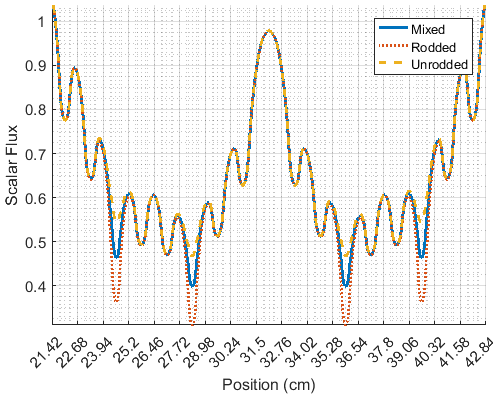
\includegraphics[width=0.7\textwidth]{../figs/1dmoc-50mix-fixedscat-scalflux7.png}
      \caption{Group 7 scalar flux comparisons for a fixed fission and scattering source calculation}\label{f:1dmoc-fixed-50-scalflux7}
    \end{figure}
    
\end{frame}

%%%%%%%%%%%%%%%%%%%%%%%%%%%%%%%%%%%%%%%%%%%%%%%%%%%%%%%%%%%%%%%%%%%%%%%%%%%%%%%%%

\begin{frame}[t]{Fixed Total Source}

\begin{figure}[H]
    \centering
    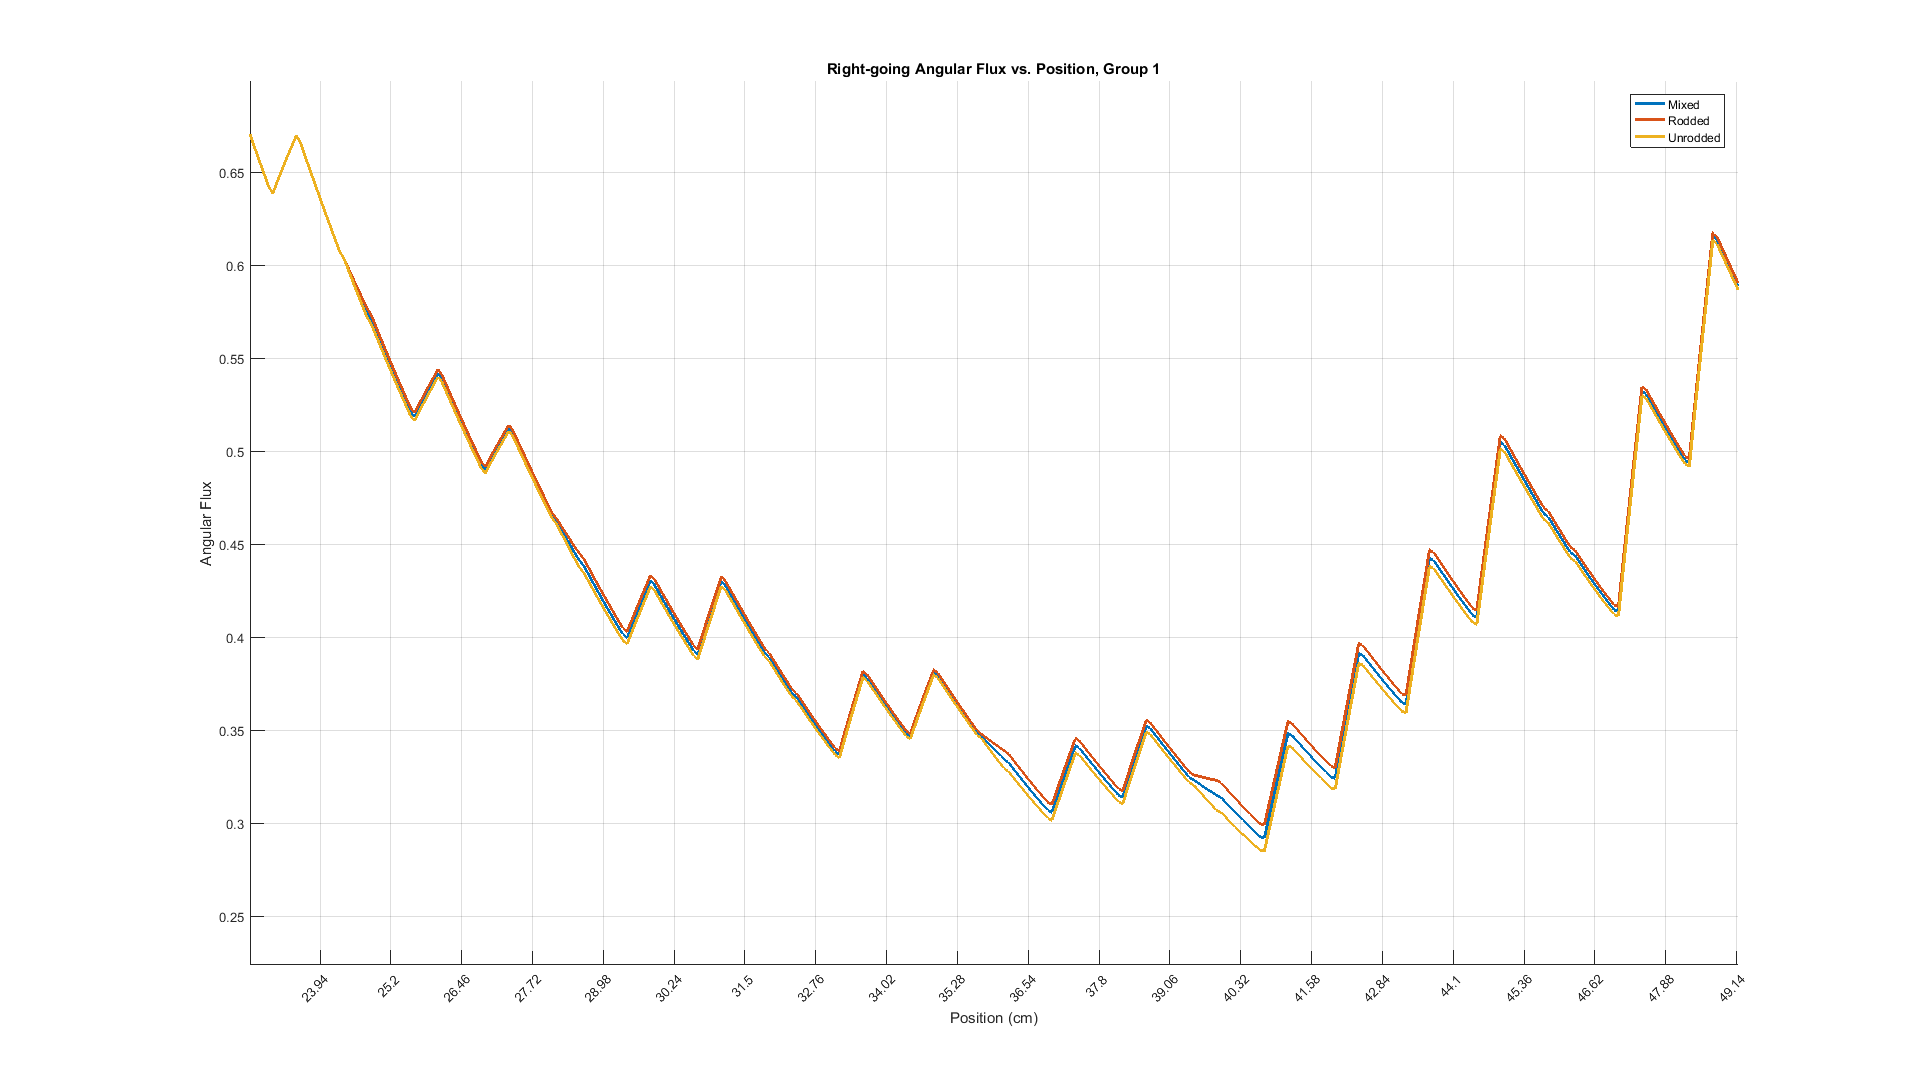
\includegraphics[width=0.6\textwidth]{../figs/1dmoc-50mix-fixedscat-angflux1.png}
\end{figure}
\begin{itemize}
  \item Fast flux differences build up
\end{itemize}

\end{frame}

%%%%%%%%%%%%%%%%%%%%%%%%%%%%%%%%%%%%%%%%%%%%%%%%%%%%%%%%%%%%%%%%%%%%%%%%%%%%%%%%%

\begin{frame}[t]{Fixed Total Source}

\begin{figure}[H]
  \centering
  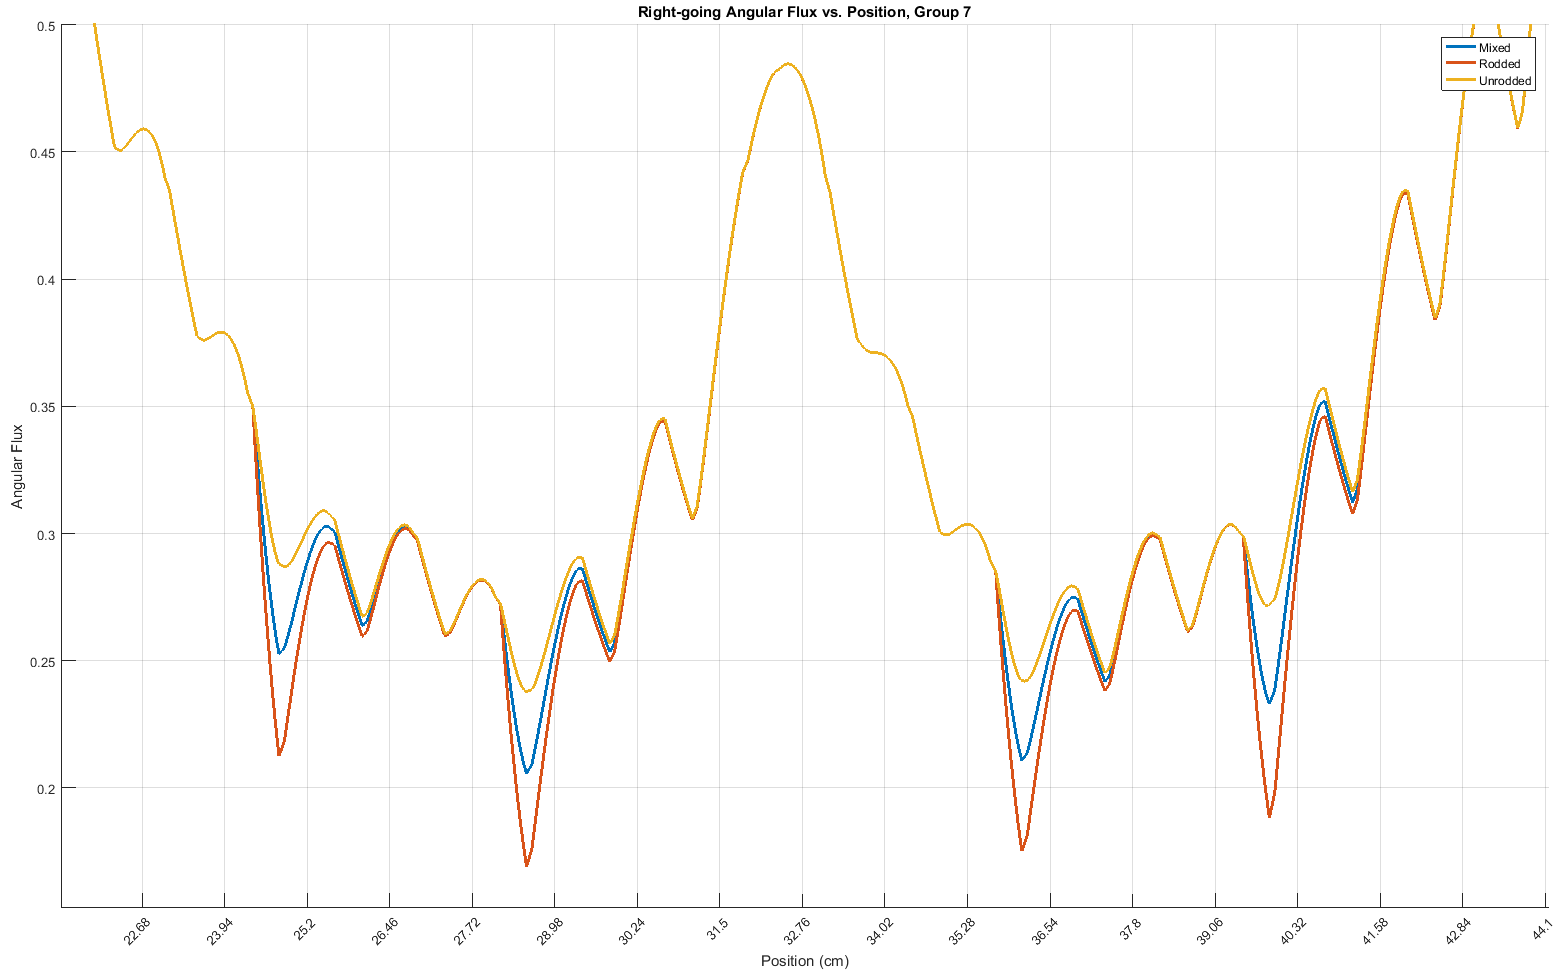
\includegraphics[width=0.6\textwidth]{../figs/1dmoc-50mix-fixedscat-angflux7.png}
\end{figure}
\begin{itemize}
  \item Thermal flux differences dissipate quickly
\end{itemize}

\end{frame}

%%%%%%%%%%%%%%%%%%%%%%%%%%%%%%%%%%%%%%%%%%%%%%%%%%%%%%%%%%%%%%%%%%%%%%%%%%%%%%%%%

\begin{frame}[t]{Fixed Fission Source}
    
    \begin{itemize}
      \item 1D model of VERA Problem 4
      \item Eigenvalue calculation performed to generate fission source
      \item Calculations performed using 25\%, 50\%, and 75\% rodded 
      cross-sections
      \begin{itemize}
        \item Same, fixed fission source for each case
        \item Multiple iterations allowed for each case to converge scattering 
        source
      \end{itemize}
    \end{itemize}
    
\end{frame}

%%%%%%%%%%%%%%%%%%%%%%%%%%%%%%%%%%%%%%%%%%%%%%%%%%%%%%%%%%%%%%%%%%%%%%%%%%%%%%%%%

\begin{frame}[t]{Fixed Fission Source}

\begin{itemize}
  \item Angular Flux, Group 7, 25\% rodded
\end{itemize}
\begin{figure}[H]
    \centering
    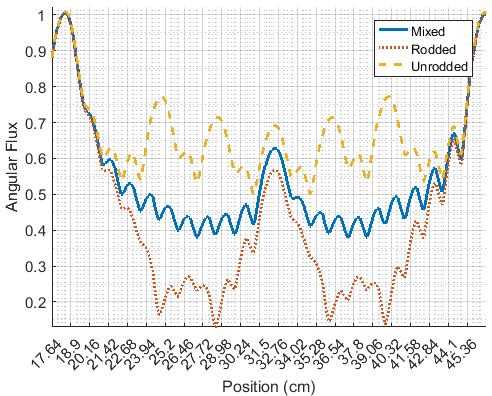
\includegraphics[width=0.6\textwidth]{../figs/1dmoc-25mix-angflux7.png}
\end{figure}

\end{frame}

%%%%%%%%%%%%%%%%%%%%%%%%%%%%%%%%%%%%%%%%%%%%%%%%%%%%%%%%%%%%%%%%%%%%%%%%%%%%%%%%%

\begin{frame}[t]{Fixed Fission Source}

\begin{itemize}
  \item Angular Flux, Group 7, 50\% rodded
\end{itemize}
\begin{figure}[H]
  \centering
  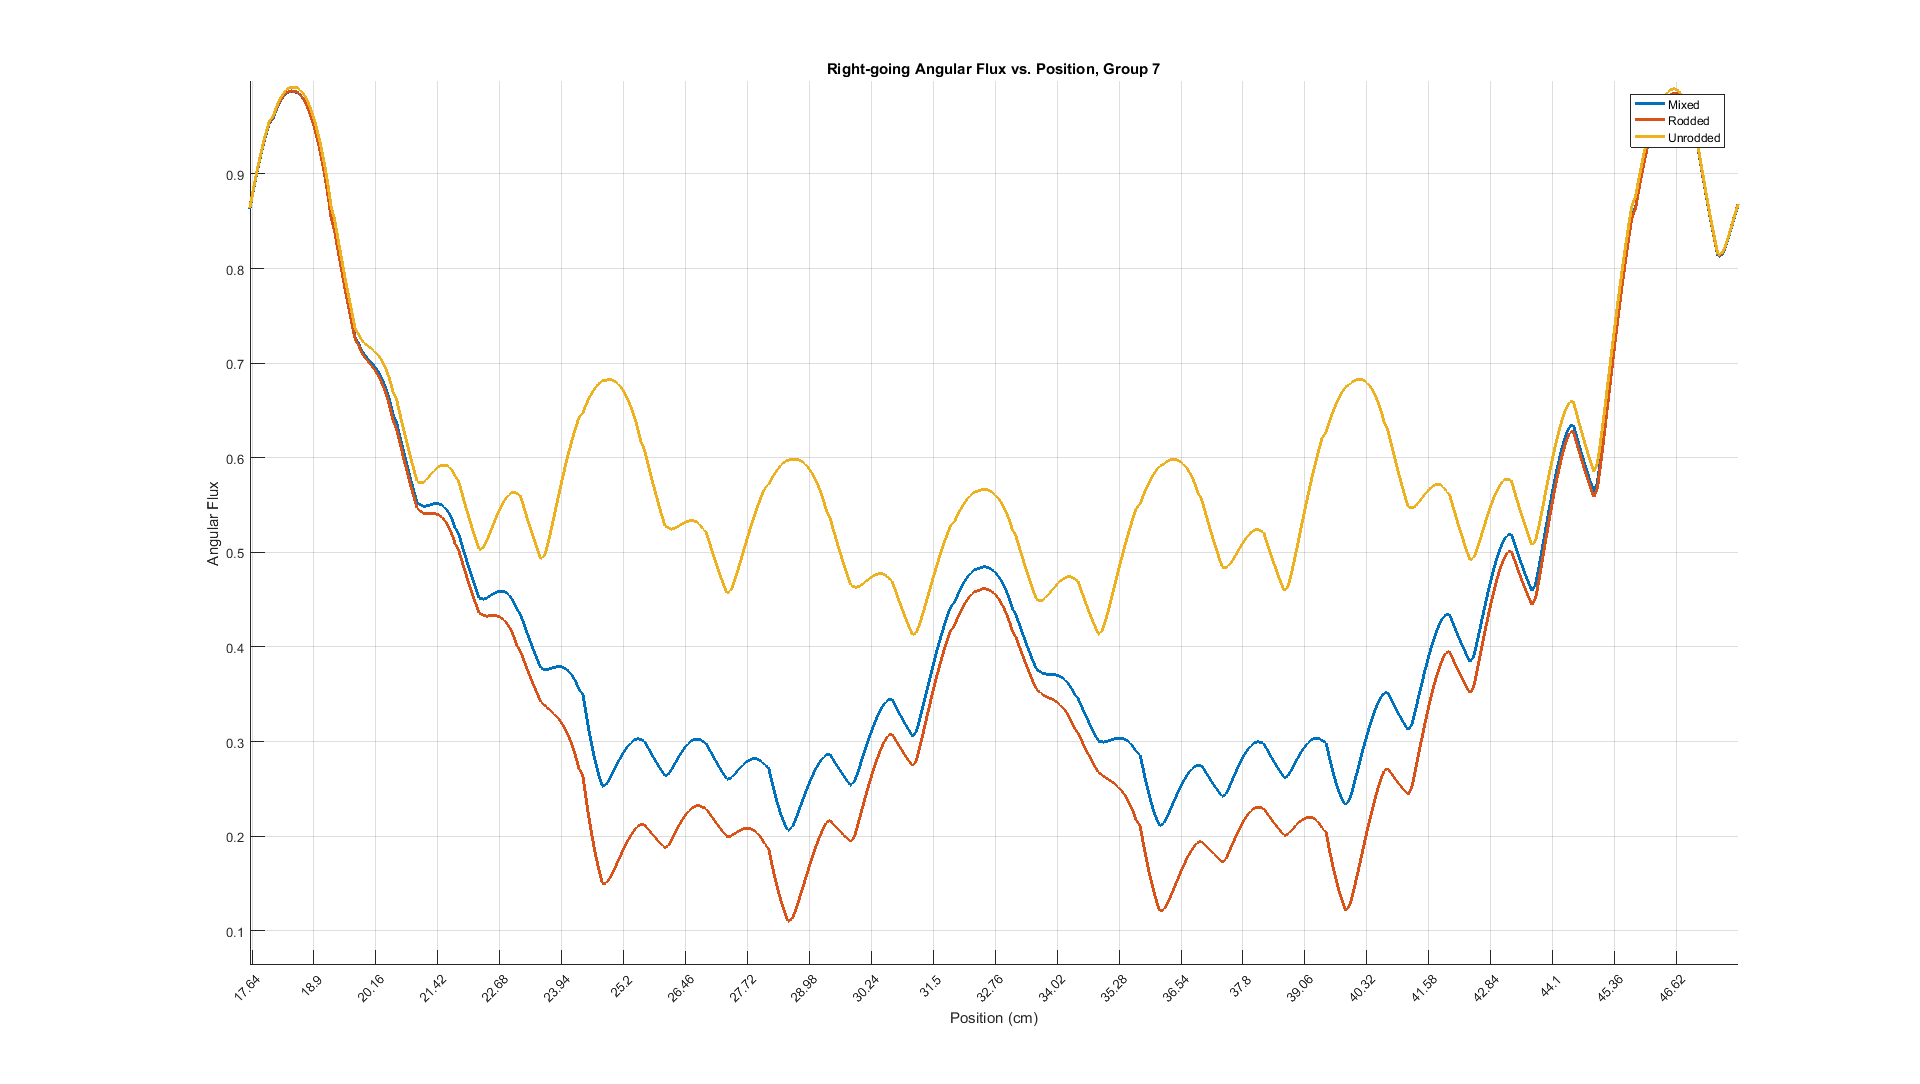
\includegraphics[width=0.6\textwidth]{../figs/1dmoc-50mix-angflux7.png}
\end{figure}

\end{frame}

%%%%%%%%%%%%%%%%%%%%%%%%%%%%%%%%%%%%%%%%%%%%%%%%%%%%%%%%%%%%%%%%%%%%%%%%%%%%%%%%%

\begin{frame}[t]{Fixed Fission Source}

\begin{itemize}
  \item Angular Flux, Group 7, 75\% rodded
\end{itemize}
\begin{figure}[H]
  \centering
  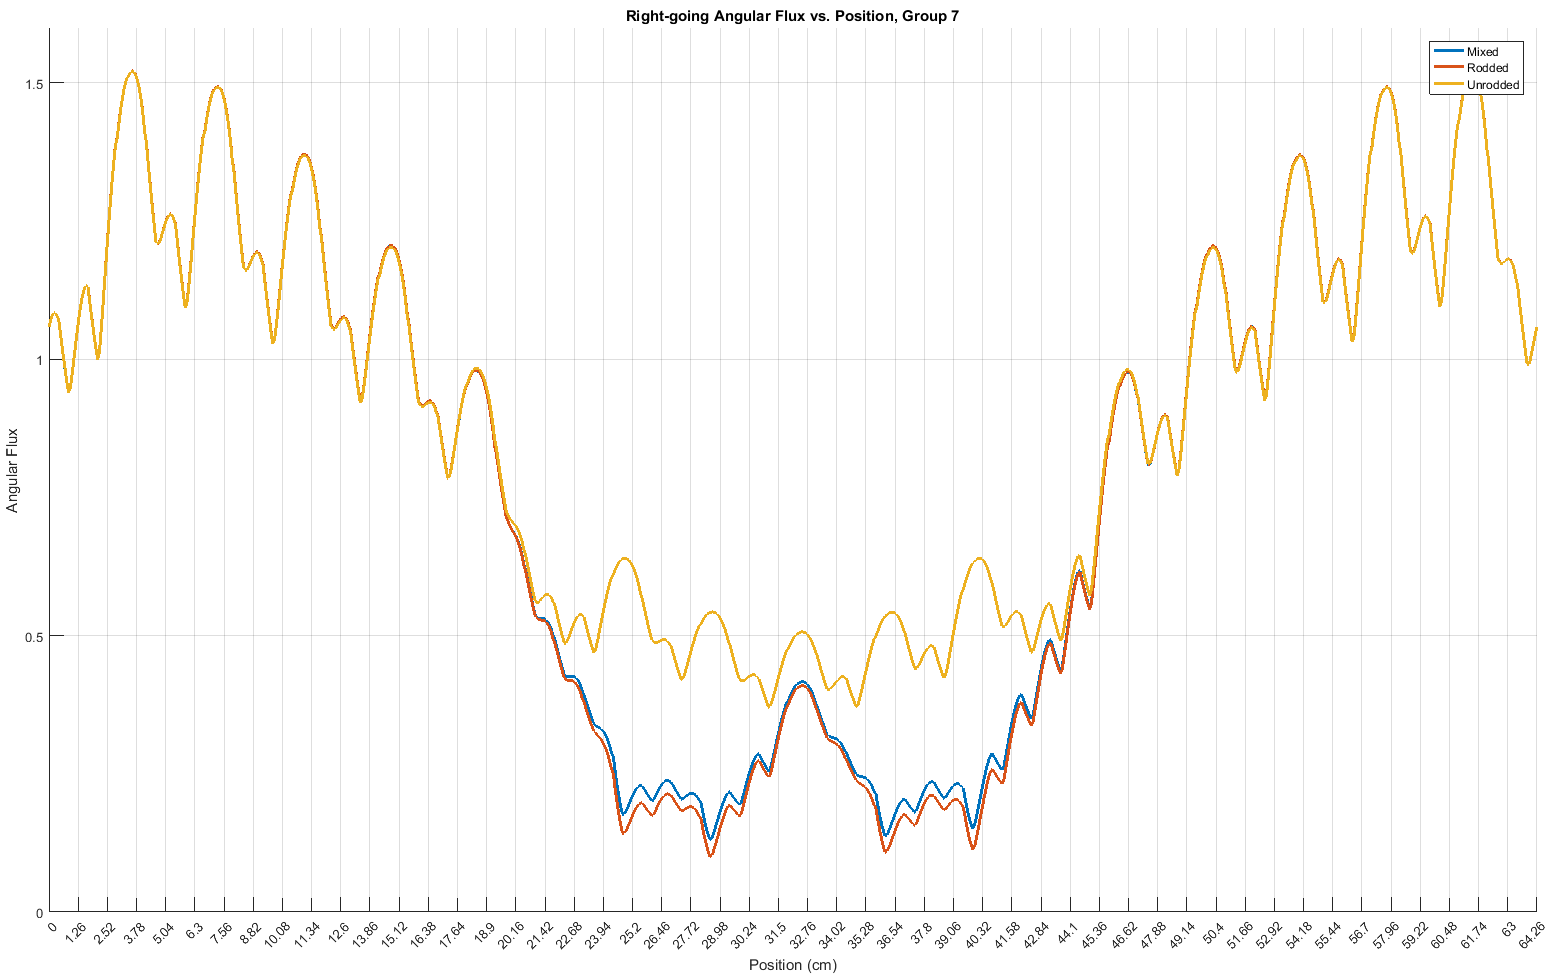
\includegraphics[width=0.6\textwidth]{../figs/1dmoc-75mix-angflux7.png}
\end{figure}

\end{frame}

%%%%%%%%%%%%%%%%%%%%%%%%%%%%%%%%%%%%%%%%%%%%%%%%%%%%%%%%%%%%%%%%%%%%%%%%%%%%%%%%%

\begin{frame}[t]{Fixed Fission Source}

\begin{itemize}
  \item Angular Flux, Group 1, 25\% rodded
\end{itemize}
\begin{figure}[H]
  \centering
  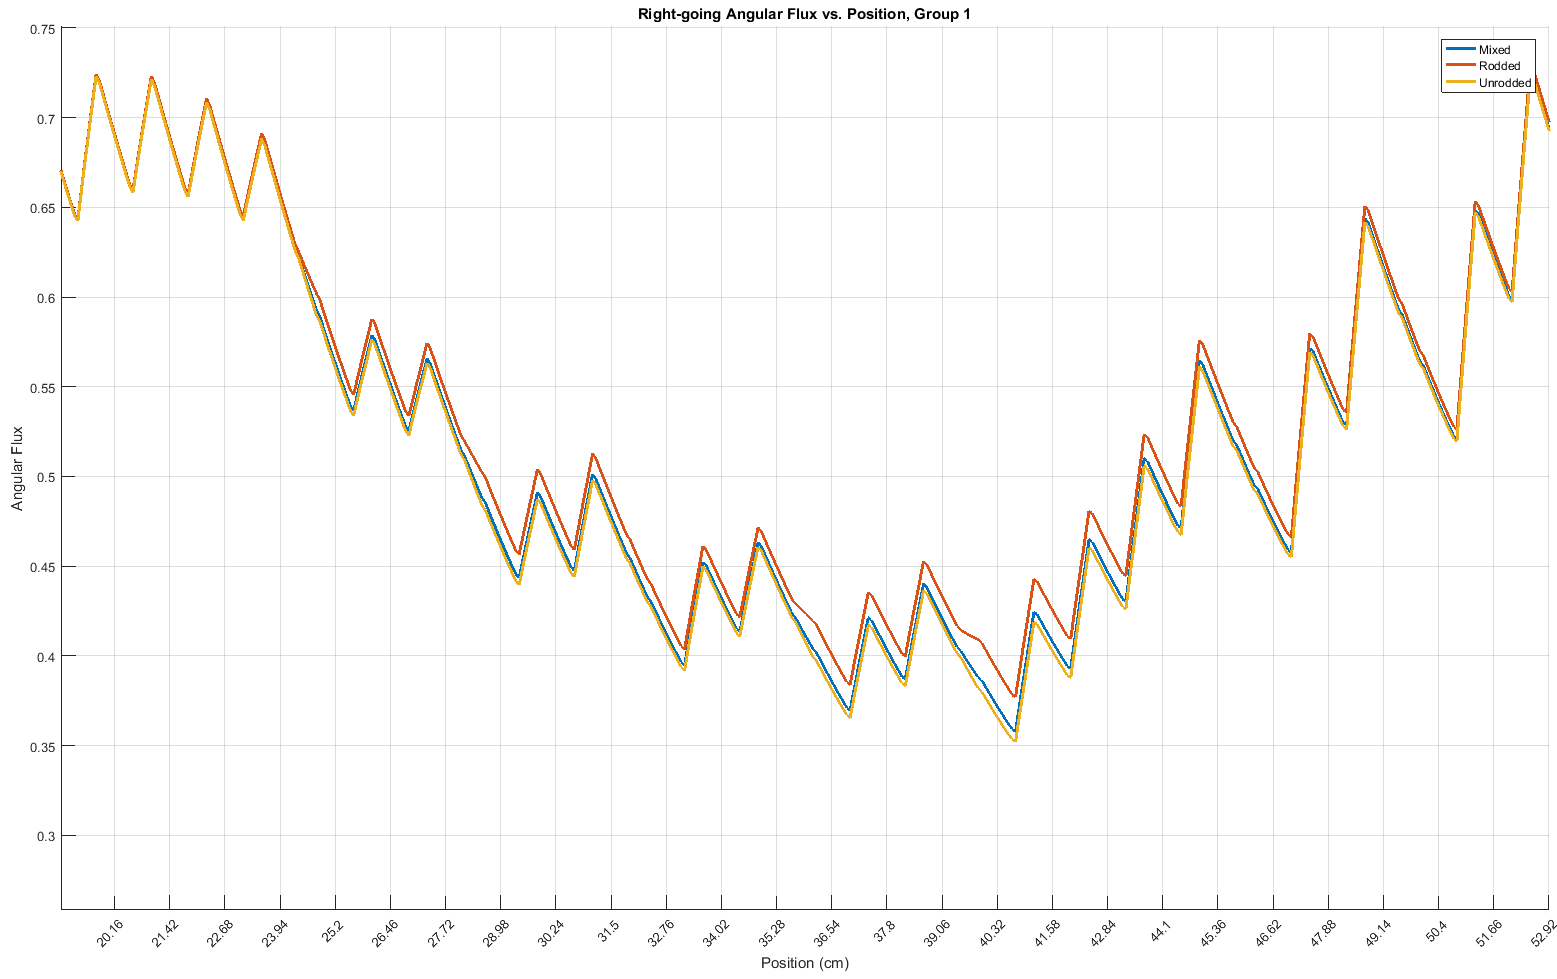
\includegraphics[width=0.6\textwidth]{../figs/1dmoc-25mix-angflux1.png}
\end{figure}

\end{frame}

%%%%%%%%%%%%%%%%%%%%%%%%%%%%%%%%%%%%%%%%%%%%%%%%%%%%%%%%%%%%%%%%%%%%%%%%%%%%%%%%%

\begin{frame}[t]{Fixed Fission Source}

\begin{itemize}
  \item Angular Flux, Group 1, 50\% rodded
\end{itemize}
\begin{figure}[H]
  \centering
  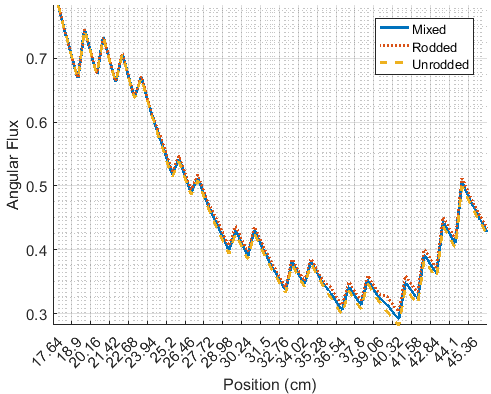
\includegraphics[width=0.6\textwidth]{../figs/1dmoc-50mix-angflux1.png}
\end{figure}

\end{frame}

%%%%%%%%%%%%%%%%%%%%%%%%%%%%%%%%%%%%%%%%%%%%%%%%%%%%%%%%%%%%%%%%%%%%%%%%%%%%%%%%%

\begin{frame}[t]{Fixed Fission Source}

\begin{itemize}
  \item Angular Flux, Group 1, 75\% rodded
\end{itemize}
\begin{figure}[H]
  \centering
  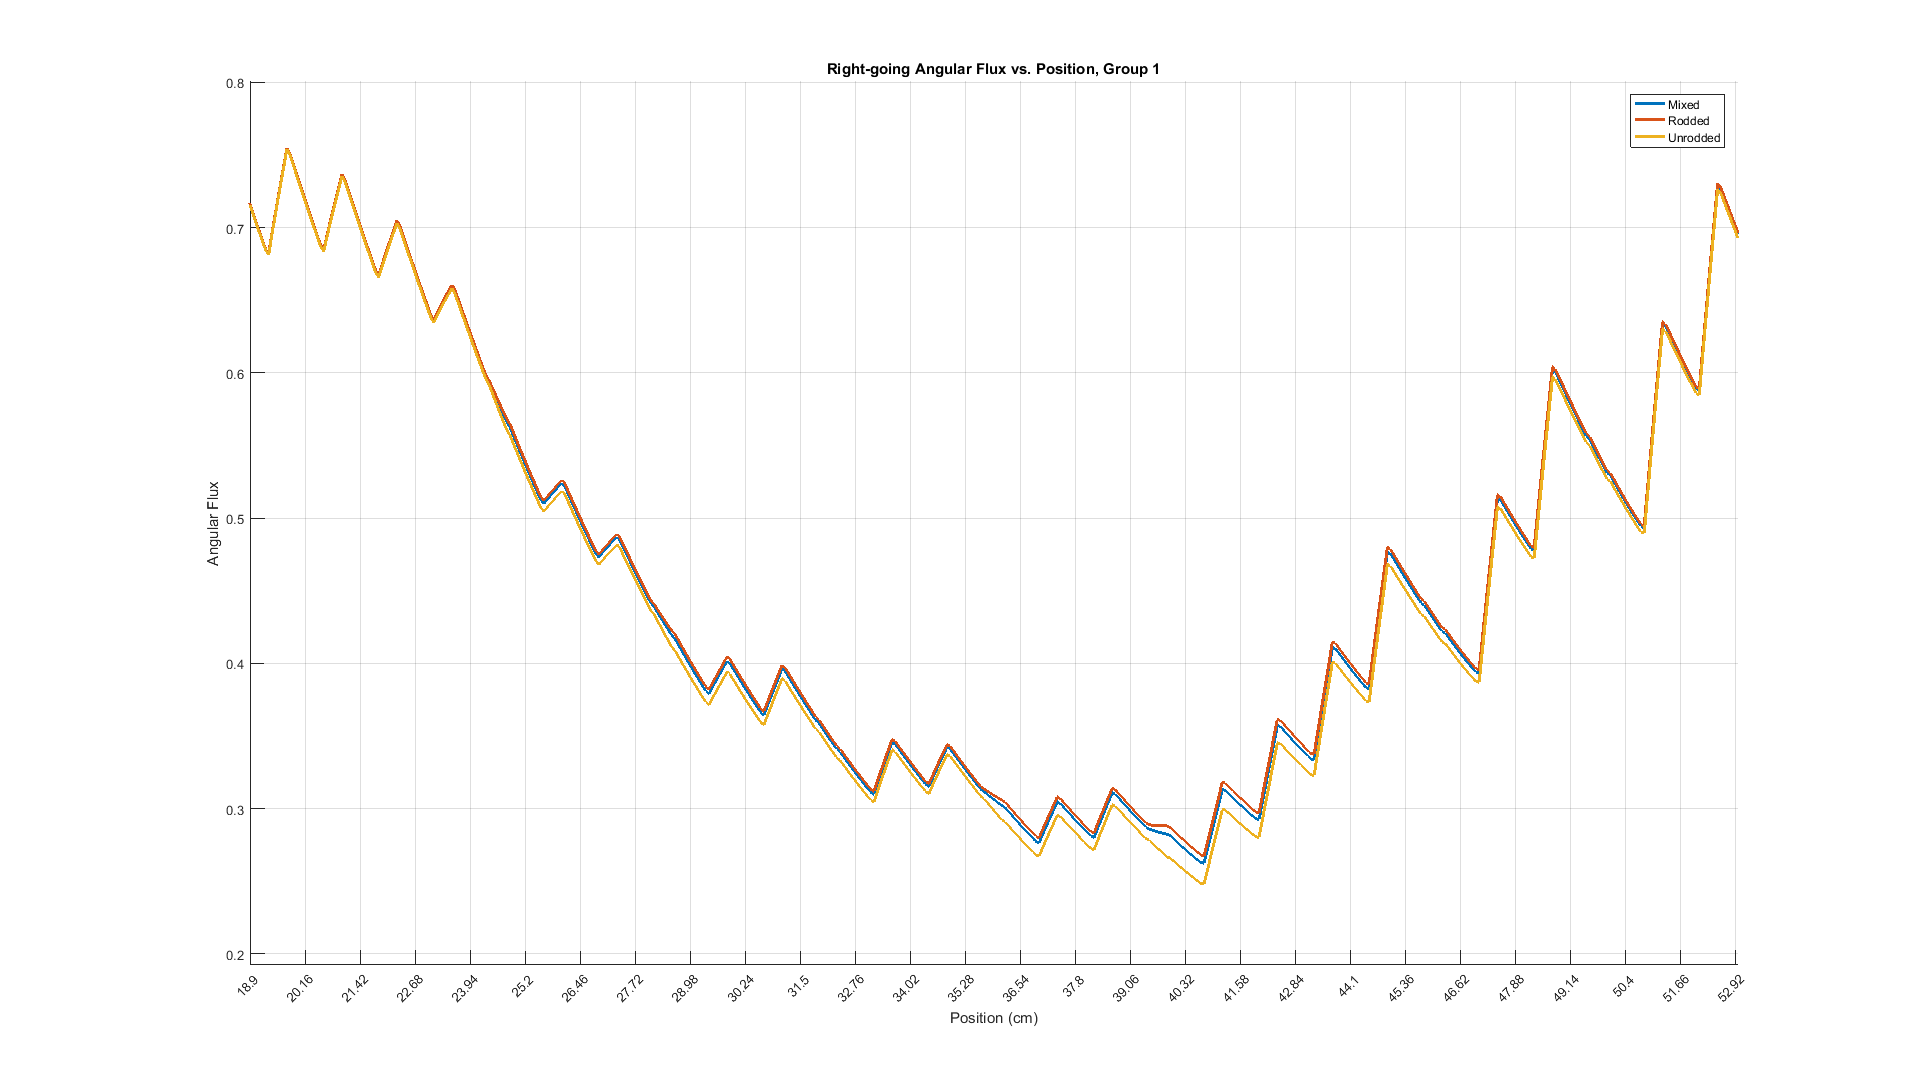
\includegraphics[width=0.6\textwidth]{../figs/1dmoc-75mix-angflux1.png}
\end{figure}

\end{frame}

%%%%%%%%%%%%%%%%%%%%%%%%%%%%%%%%%%%%%%%%%%%%%%%%%%%%%%%%%%%%%%%%%%%%%%%%%%%%%%%%%

\begin{frame}[t]{Discussion}
    
    
    
\end{frame}

%%%%%%%%%%%%%%%%%%%%%%%%%%%%%%%%%%%%%%%%%%%%%%%%%%%%%%%%%%%%%%%%%%%%%%%%%%%%%%%%%

\begin{frame}[t]{Sub-Ray MOC Method}
    
    
    
\end{frame}